\documentclass{article}
\usepackage{polski}
\usepackage[utf8]{inputenc}
\usepackage{graphicx}
\usepackage{placeins}
\usepackage{siunitx}
\usepackage{svg}
\sisetup{math-micro=\text{µ},text-micro=µ}
\graphicspath{ {./img/} }

\title{Regresja liniowa i drzewa decyzyjne}
\author{Piotr Kumala}
\date{09.06.2022 r.}

\begin{document}
	
	\maketitle
	
	\section{Wstęp}
	W tym dokumencie przedstawione zostanie zastosowanie klasycznych metod predykcji szeregów czasowych, otrzymane wyniki oraz wnioski z nich płynące. Uzyskane wyniki zostaną wykorzystane jako wartości referencyjne przy analizie skuteczności zastosowań rekurencyjnych sieci neuronowych do tego samego problemu. W podsumowaniu przedstawiony zostanie również dalszy kierunek prowadzonych prac oraz ostateczny cel tychże badań. 
	
	\section{Wybór danych do dalszej analizy}
	W trakcie przeprowadzania regresji liniowej zauważono, że przygotowany wcześniej zbiór danych o wypadkach rowerowych w Wielkiej Brytanii niestety nie jest odpowiedni do przeprowadzania na nim predykcji. Każdy wypadek posiada informacje o warunkach pogodowych, oświetleniu, porze dnia i rodzaju drogi. Nie można jednak na podstawie żadnej z tych charakterystyk prowadzić wnioskowania o ilości wypadków danego dnia. Nie został przygotowany szereg czasowy opisujący te cechy, a stworzenie go jest bardzo skomplikowane o ile w ogóle wykonalne. 
	Z tego powodu podjęta została decyzja o porzuceniu tych danych i skupieniu dalszej pracy nad danymi klimatyczno-pogodowymi Krakowa w latach 2000-2021. W pracy nad tymi danymi nie zauważono żadnych znaczących problemów i wydaje się, że są one odpowiednie do prowadzenia dalszych badań. 
	
	
	\section{Regresja liniowa}
	Przeprowadzona została regresja liniowa gdzie na podstawie minimalnej temperatury gruntu, dziennej sumy opadów oraz maksymalnej, minimalnej i średniej dziennej temperatury estymowana był średni dzienny poziom zanieczyszczenia pyłem PM10. 
	
	Dane zostały podzielone na zbiory trenujący i testujący, a następnie przeprowadzona została najprostsza regresja liniowa. W jej wyniku otrzymaliśmy błąd średniokwadratowy równy 1386.290 [$\frac{\si{\micro\gram}}{\si\meter^3}$] oraz wynik testu $R^2$ równy 0.323. Sporządzony został również wykres przewidywanego oraz rzeczywistego poziomu zanieczyszczenia pyłem PM10:
	\begin{figure}[!ht]
		\centering
		\makebox[0pt]{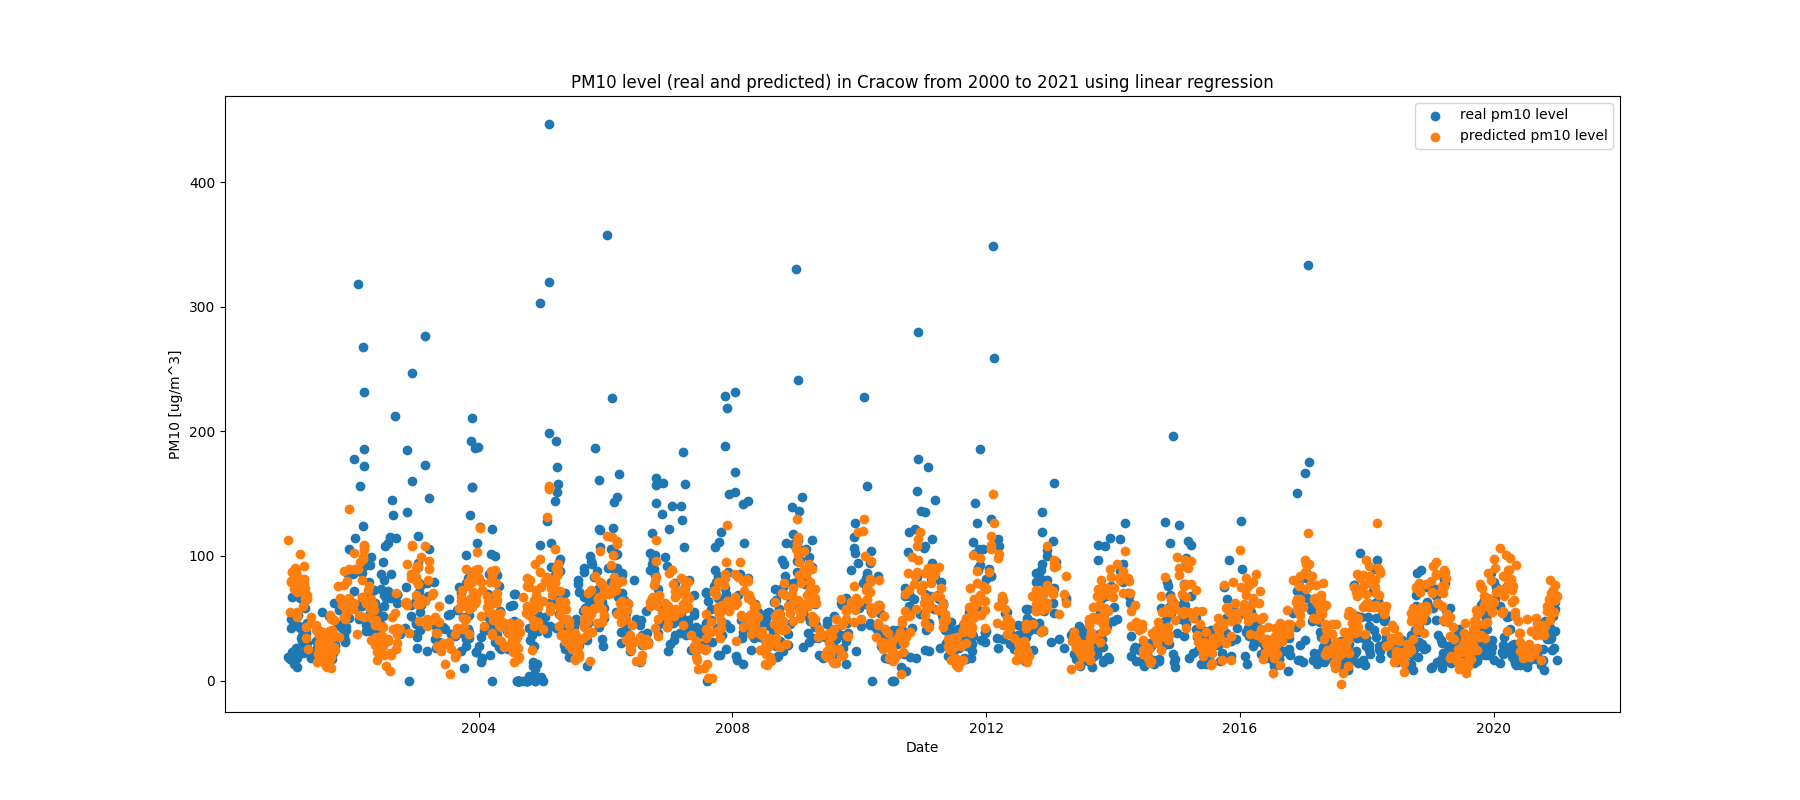
\includegraphics[scale=0.35]{linear_regression}}
		\caption{Wyniki regresji liniowej}
	\end{figure}
	\FloatBarrier
	
	\section{Drzewo decyzyjne}
	Przeprowadzona została również regresja z wykorzystaniem drzewa decyzyjnego na podstawie tych samych cech co w poprzedniej metodzie. 
	
	W trakcie przeprowadzania regresji zauważono tendencję drzewa decyzyjnego do zbytniego dopasowywania(overfitting) do danych trenujących sprawiającą, że wynik $R^2$ był ujemny. 
	Aby zaradzić temu problemowi została zmniejszona maksymalna głębokość drzewa decyzyjnego, po serii prób za najlepszą wartość maksymalnej głębokości uznano 3. Przy takiej konfiguracji drzewa decyzyjnego otrzymany został wynik $R^2$ równy 0.311 oraz błąd średniokwadratowy równy 1409.991 [$\frac{\si{\micro\gram}}{\si\meter^3}$].
	\begin{figure}[!ht]
		\centering
		\makebox[0pt]{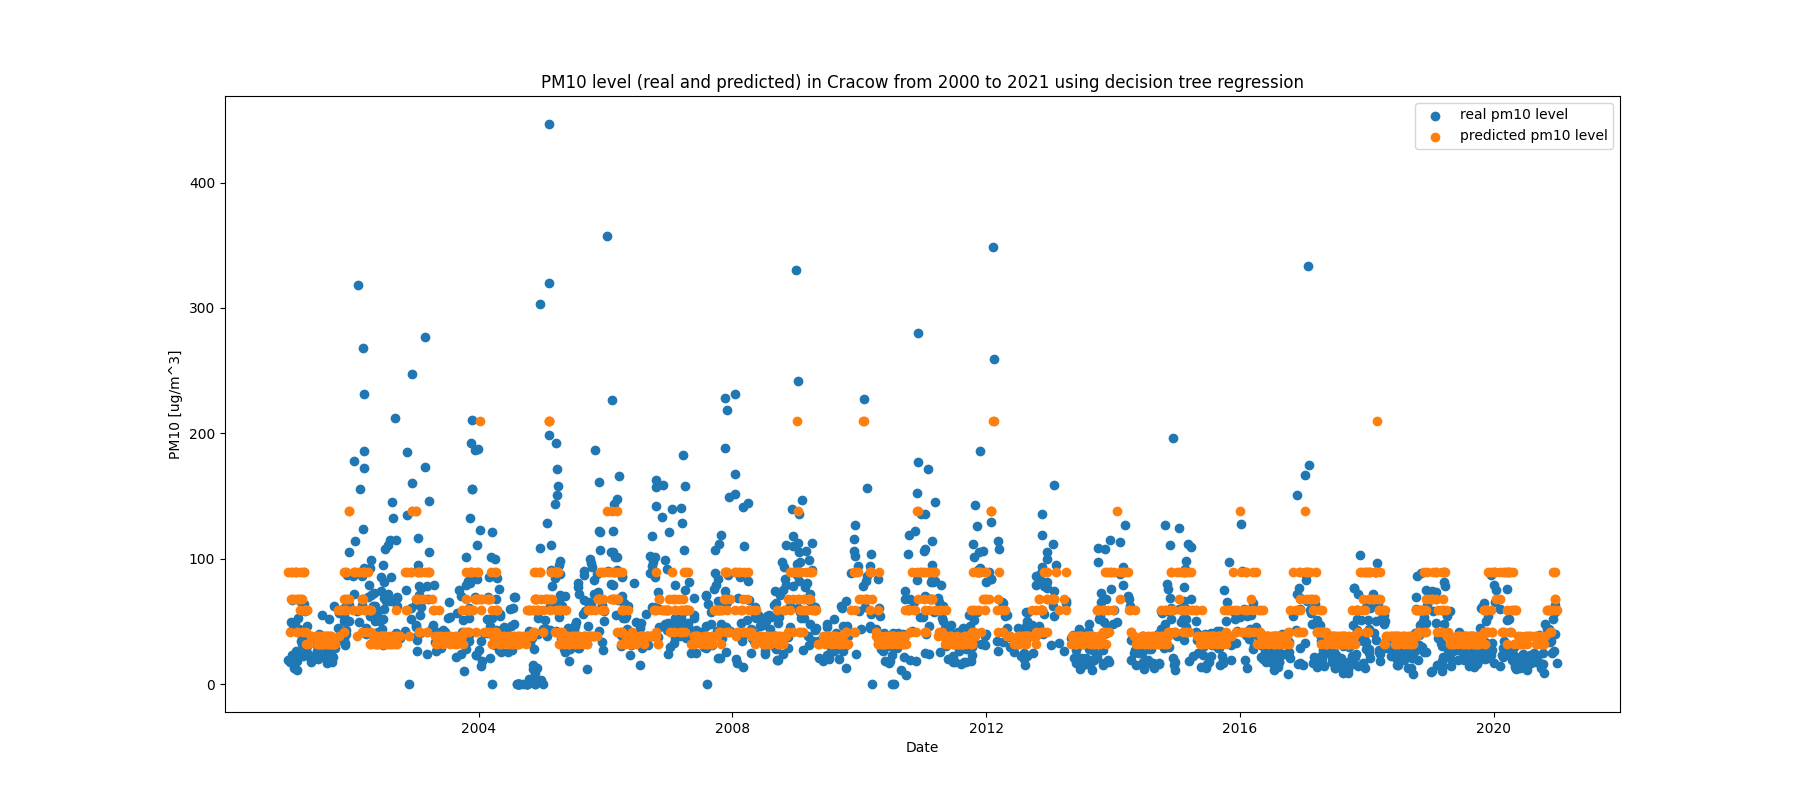
\includegraphics[scale=0.35]{decision_tree}}
		\caption{Wyniki regresji z wykorzystaniem drzewa decyzyjnego}
	\end{figure}
	\FloatBarrier
	Stworzona została również wizualizacja drzewa decyzyjnego.
	\begin{figure}[!ht]
		\centering
		\makebox[0pt]{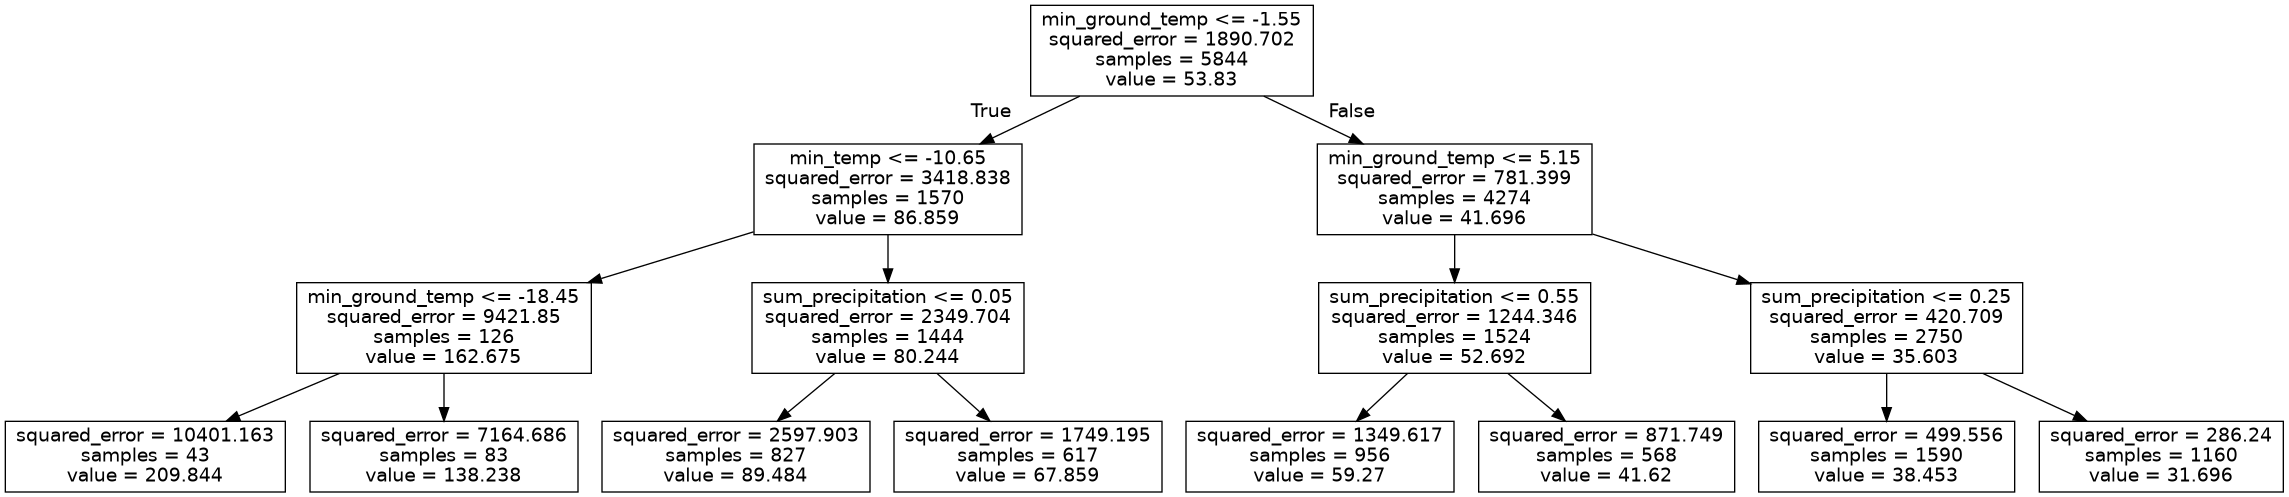
\includegraphics[scale=0.25]{tree}}
		\caption{Wizualizacja drzewa decyzyjnego}
	\end{figure}
	\FloatBarrier
	
	\section{Wnioski}
	Na podstawie przeprowadzonej regresji wydaje się, że przygotowane dane są odpowiednie do dalszej analizy z wykorzystaniem rekurencyjnych sieci neuronowych. Podczas dalszych badań będzie trzeba zwracać uwagę na problem zbytniego dopasowywania, który uwydatnił się przy regresji z wykorzystaniem drzewa decyzyjnego. Planowane jest przeprowadzenie predykcji z wykorzystaniem podstawowej rekurencyjnej sieci neuronowej, sieci LSTM oraz GRU. Końcowym celem badań jest ewaluacja przydatności rekurencyjnych sieci neuronowych do predykcji szeregów czasowych poprzez porównanie wyników wszystkich używanych metod. Interesujące może się również okazać porównanie wyników różnych sieci neuronowych, na przykład sieci LSTM i GRU. Sieć GRU jest często przedstawiana jako mniej skomplikowana alternatywa uzyskująca porównywalne wyniki. Określenie czy w naszym konkretnym zastosowaniu zaobserwujemy taką charakterystykę może być badawczo ciekawe.
\end{document}